\documentclass[10pt]{article}

\usepackage{siunitx}
\usepackage{amsmath}
\usepackage{amsfonts}
\usepackage{booktabs}
\usepackage[margin=0.75in]{geometry}
\usepackage{graphicx}

\renewcommand{\vec}{\mathbf}
\newcommand{\R}{\mathbb{R}}


\begin{document}
  \begin{tabular}{l}
    Box Num. 33 \\
    Problem Set 31 \\
    \today
  \end{tabular}

  \begin{enumerate}
    \item The energy of any given wave must be
    \begin{equation*}
        E = pc = c\sqrt{p_x^2 + p_y^2}.
    \end{equation*}
    Since every momentum component must be consistent with the boundary conditions for that wavelength,
    \begin{equation*}
        E = c\sqrt{\left(\frac{\hbar \pi n_x }{L}\right)^2 + \left(\frac{\hbar \pi n_y }{L}\right)^2} =
        \frac{\hbar c \pi}{L}\sqrt{n_x^2 + n_y^2} = \frac{\hbar c n \pi}{L}
    \end{equation*}
    Since there are only two dimensions in this problem (instead of three as shown in class), we need to imagine a disk instead of a sphere. The number of points corresponding to a value of $E$ is then $\frac{1}{2} \pi n$, where $n= \sqrt{n_x^2+n_y^2}$. Since there are two possible spins for photons, the number of states per unit volume is
    \begin{equation*}
        g(n)dn = \frac{1}{2} \frac{2}{A} \pi n dn = \frac{\pi n}{L^2} dn = g(E)dE
    \end{equation*}
    Since $E=\frac{\hbar c n \pi}{L}$, we have $dE = \frac{\hbar c \pi}{L}$, so $g(E) = \frac{n}{cL\hbar}$.

    \item The Maxwell-Boltzmann energy distribution for this gas of electrons is
    \begin{equation*}
        g(E) = \frac{2}{\sqrt{\pi} (kT)^{3/2}}E^{1/2}e^{-E/kT} =
        \frac{2}{\sqrt{\pi} (\SI{0.0252}{\electronvolt})^{3/2}} E^{1/2} e^{-E/\SI{0.0252}{\electronvolt}}
    \end{equation*}
    The interval of 1\% around the most probable energy is the range from $\SI{.02495}{\electronvolt}$ to $\SI{0.2545}{\electronvolt}$. According to the Stefan-Boltzmann distribution, the

  \item[4.] \begin{enumerate}
      \item The partition function is defined as:
      \begin{equation*}
          Z = \sum_{i}e^{-E_i/k_B T} = e^{-\epsilon/k_B T} + 2e^{0} + e^{\epsilon/k_B T} = 2 + e^{\epsilon/k_B T} + e^{-\epsilon/k_B T}
      \end{equation*}

      \item The probability of the system having energy 0 is
      \begin{equation*}
          P_0 = \frac{2}{2 + e^{\epsilon/k_B T} + e^{-\epsilon/k_B T}}
      \end{equation*}
      And the probability that it has energy $\epsilon$ or $-\epsilon$, respectively, is
      \begin{equation*}
          P_{\epsilon} = \frac{E^{-\epsilon/k_B T}}{2 + e^{\epsilon/k_B T} + e^{-\epsilon/k_B T}},
          P_{-\epsilon} = \frac{E^{\epsilon/k_B T}}{2 + e^{\epsilon/k_B T} + e^{-\epsilon/k_B T}}
      \end{equation*}

      \item These figures show the probabilities of $E=0$, $E=\epsilon$, and $E=-\epsilon$, respectively.

      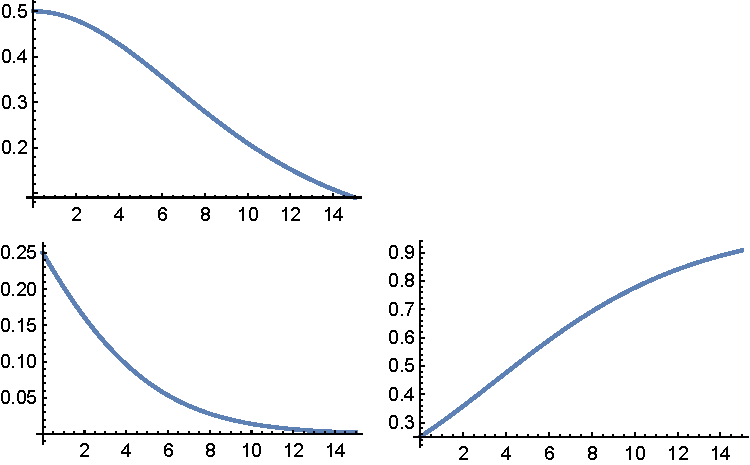
\includegraphics{p314cgraphs}
  \end{enumerate}
  \end{enumerate}
\end{document}
